\documentclass{gescons}

\genre {Atualizações}
\author{Ana Claudia Prado e~Ana Mazzonetto}
\authorrole{Editoras da Revista Editares}
\title{Editares Lança Revista Científica Especializada em Editoriologia e~Publicaciologia}

\begin{document}
    \makeentrevistatitle
    %\maketitle

    %\fullwidthimage{fields}{b}

    %\coverart{back/editorial}
    \coverart{../fundo-generico}
    
    
\begin{center}
    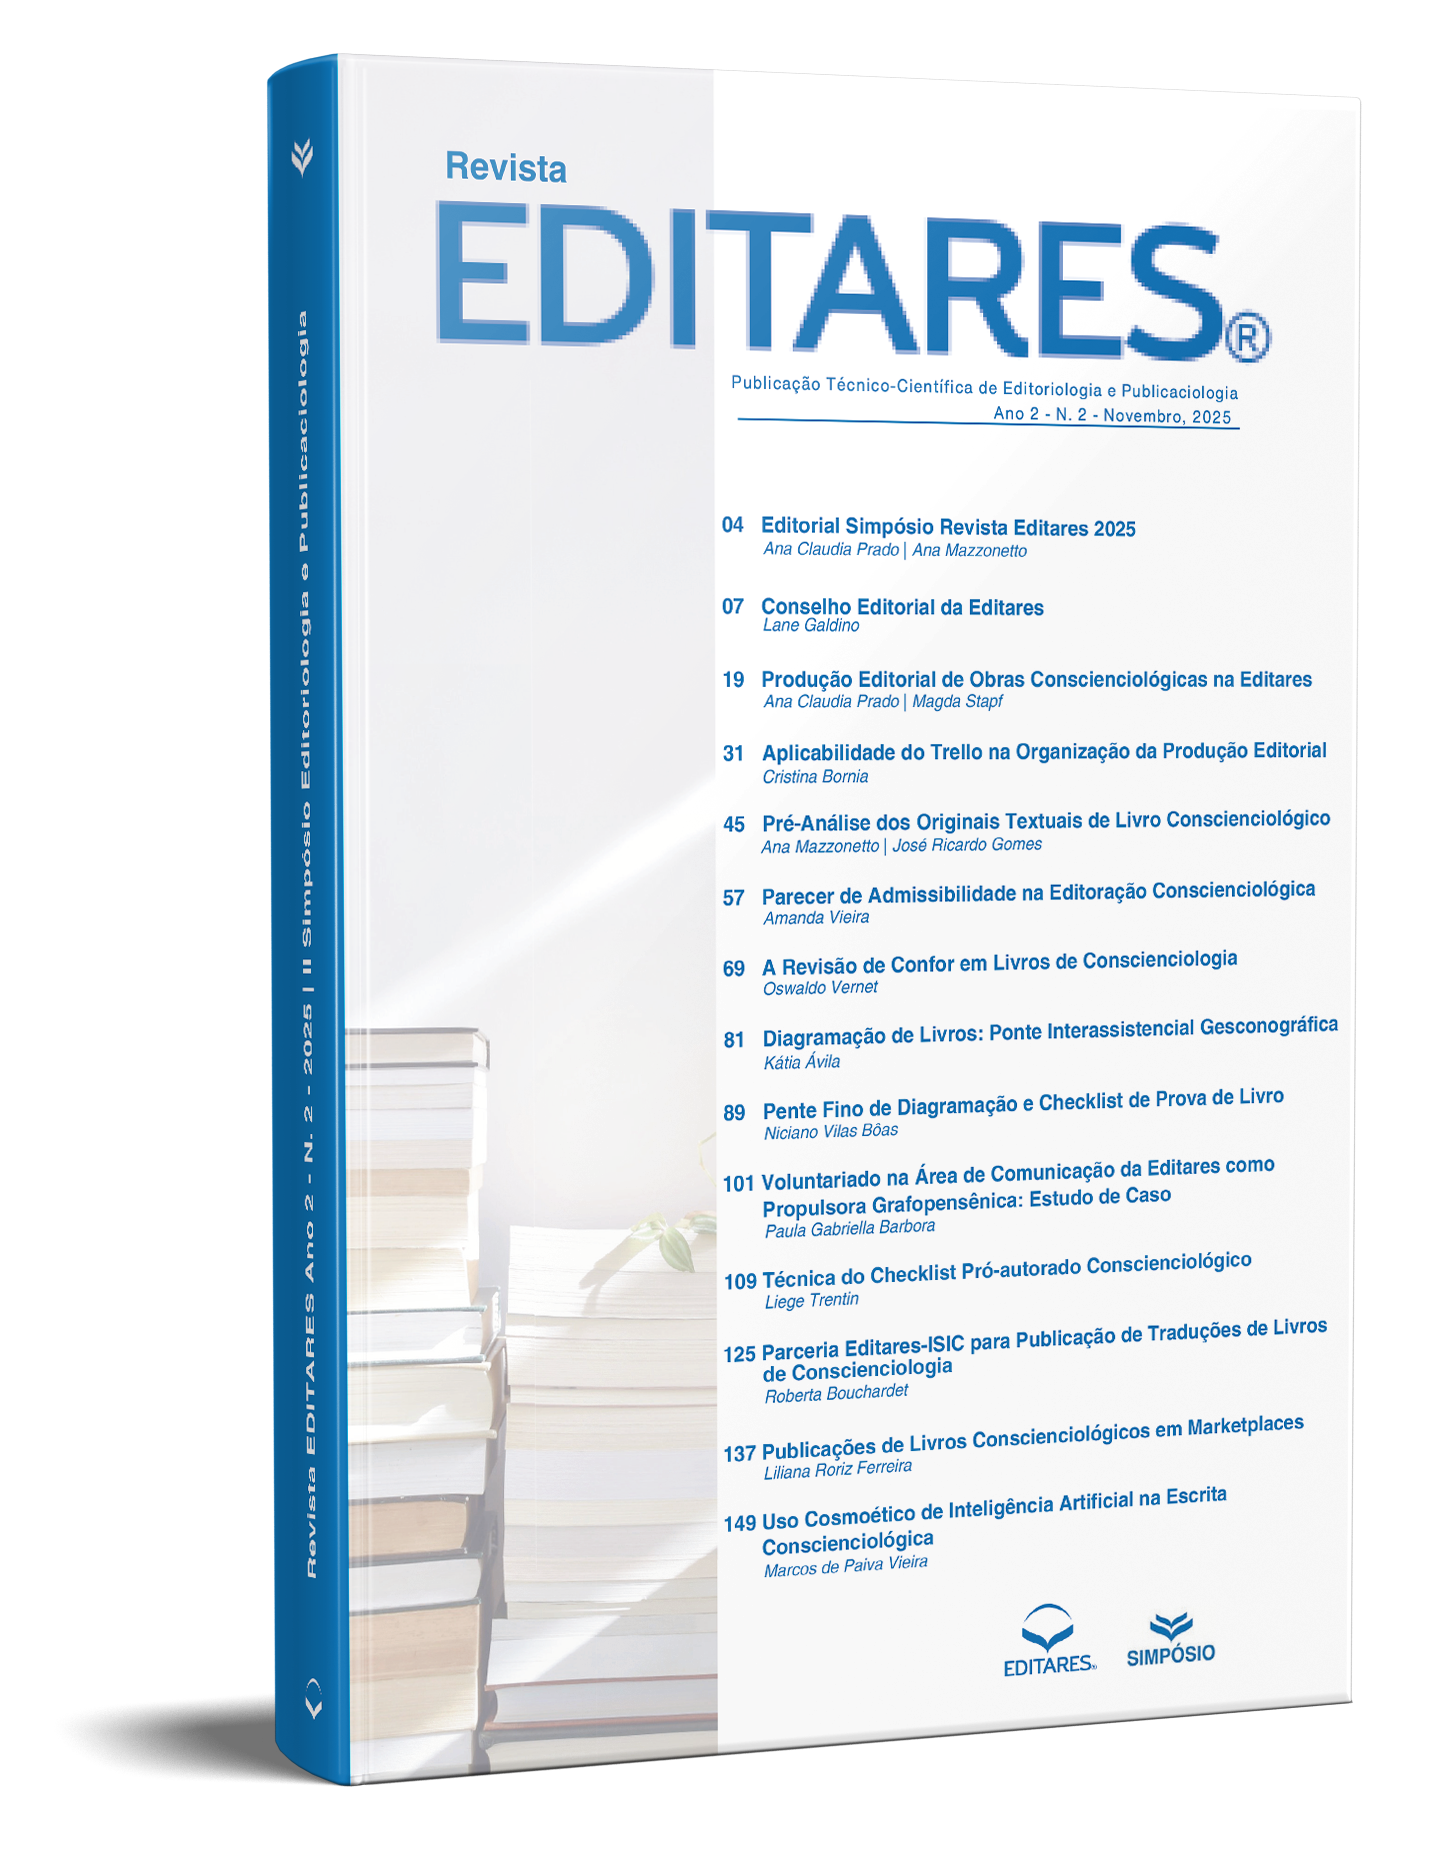
\includegraphics[height=10cm]{articles/atualizacoes/fotos/materia6/revista_editares_2025} 
\end{center}
    
    \begin{multicols}{2}


A Associação Internacional Editares, dedicada à~editoração e~publicação de gestações conscienciais, anunciou em novembro de 2025 o~lançamento da \textbf{Revista Editares,} publicação científica voltada exclusivamente às especialidades de \emph{Editoriologia e~Publicaciologia.} O~lançamento ocorreu durante evento temático sobre essas áreas de estudo: \textbf{II Simpósio Editoriologia e~Publicaciologia.}

A novidade representa um avanço em relação à~edição especial da \emph{Revista Gescons} nº 5, publicada em 2023, quando voluntários da Editares apresentaram, por meio de artigos científicos, os bastidores da produção editorial conscienciológica.

A escolha de um novo nome não se restringe a~uma mudança formal. A~decisão editorial visa demarcar, de modo preciso, o~\textbf{caráter científico da publicação} e~a~construção de novos conhecimentos a~partir de artigos técnicos nas duas especialidades.

Com a~criação da \emph{Revista Editares,} a~instituição passa a~separar claramente os campos de atuação: enquanto a~nova publicação concentra análises científicas, a~\emph{Revista Gescons} continua sendo o~espaço destinado ao registro de lançamentos de livros e~outras pontuações editoriais e~administrativas.

A iniciativa reforça o~compromisso da Editares com o~profissionalismo editorial, legitima processos mais exigentes de revisão por pares, fortalece a~especialização temática e~consolida a~identidade científica da instituição.

O segundo número da \emph{Revista Editares} reúne \textbf{treze artigos inéditos,} abordando desde os meandros do fluxo editorial até as vivências dos voluntários no processo de editoração e~publicação de obras conscienciológicas, sempre à~luz do Paradigma Consciencial.

\emph{``Este é~um momento de atualização do processo editorial da Editares, no qual reafirmamos publicamente nosso compromisso com a~produção científica nas especialidades de Editoriologia e~Publicaciologia'',} ressaltam as editoras Ana Claudia Prado e~Ana Mazzonetto.



%\emph{Editoras da Revista Editares}

%\emph{{[}Foto das autoras{]}}

%\emph{{[}INSERIR MOCKUP DA REVISTA QUE ESTÁ NA PASTA MATÉRIA 6{]}}


%\begin{center}
%    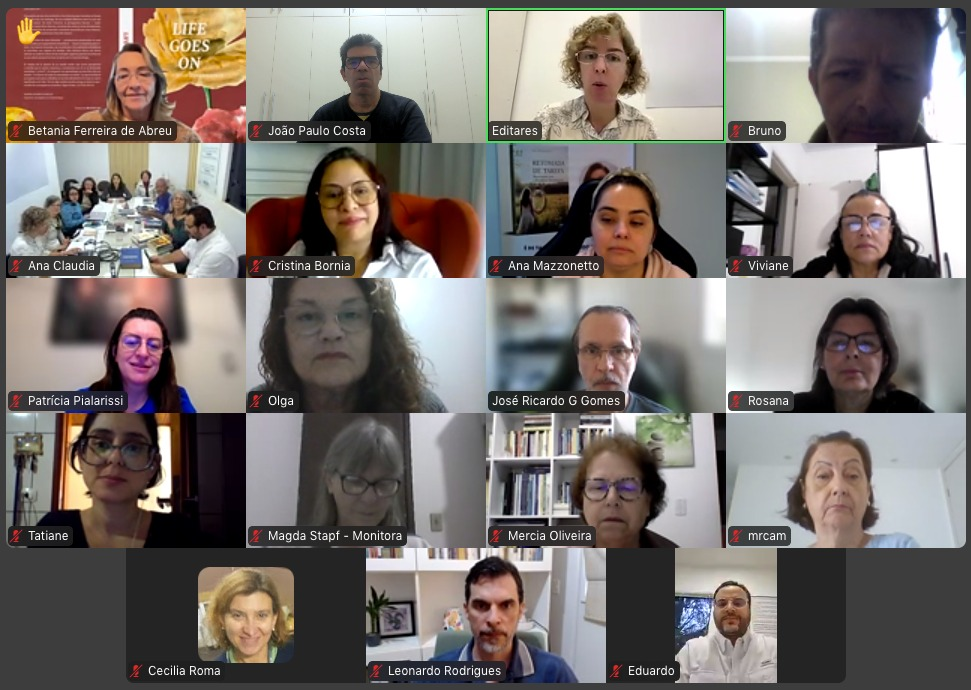
\includegraphics[width=9cm]{articles/atualizacoes/fotos/escola-editores/escola-editores1.jpeg} 
%\end{center}


    \end{multicols}
\end{document}


